% Note that the text in the [] brackets is the one that will
% appear in the table of contents, whilst the text in the {}
% brackets will appear in the main thesis.

%% CHAPTER HEADER /////////////////////////////////////////////////////////////////////////////////////
\chapter[Parameter study of \ac{gw} propagation in \ac{hsc}]{Parameter study of \ac{gw} propagation in \ac{hsc}}
\label{ch:tempEffects}

%% CHAPTER INTRODUCTION ///////////////////////////////////////////////////////////////////////////////
In the chapter~\ref{ch:severity}, the \ac{madif} was determined for the sample at ambient temperature of \(+20^{\circ}\)C.
However, quasi-stable conditions can only be guaranteed in a laboratory.
Therefore, from a practical point of view, it is necessary to consider changes due to different working conditions.
In this chapter, a study will be carried out to determine the effect of various ambient temperature on the \ac{madif}.
In addition, a series of computer simulations will be performed to determine how the different parameters of the \ac{hsc} components affect the wave propagation in this structure.
The analysis will include factors such as the adhesive thickness, the \ac{pzt} placement regarding the core cell, the core orientation regarding the wave propagation and fibre volume fraction.
Finally, the \ac{madif} will be developed for \ac{hsc} with the skins on the top and bottom sides of the core.
%% INCLUDE SECTIONS ///////////////////////////////////////////////////////////////////////////////////
%% SECTION HEADER /////////////////////////////////////////////////////////////////////////////////////
\section{The \acs{madif} under variable temperature conditions}
\label{sec:madifTemp}

%% SECTION CONTENT ////////////////////////////////////////////////////////////////////////////////////
In addition to the referenced \ac{madif} obtained for +20\unit{\degreeCelsius}, a study of wave propagation at temperatures T=\(\left[-10,\,0,\,+10,\,+30,\,+40,\,+50\right]\)\unit{\degreeCelsius} was carried out.
To determined temperature-dependent simulations of \ac{gw} propagation in \ac{hsc}, the material properties of the components were determined according to the methodology described in section~\ref{sec:temp}.

The temperature effect on the \acp{madif} is developed based on the \ac{fcgm} and removed core cells as a damage model.
The analysis used both \acp{di}, i.e. the \ac{rmsd} and the \ac{cc}, for the 100 \unit{\kHz} full-length signal.
The signal obtained for a healthy sample at each temperature was taken as the reference signal for each case.
\begin{table}[!tbh]
	\small
	\tabcolsep=0.25cm
	\centering
	\caption{\label{tab:fit_F_err_temp} The time-dependent coefficients and errors of the function from Eq.~(\ref{eq:function_1}) fitted to \acp{di} based on the \acf{fcgm} - core.}
\begin{tabular}{c|cc|cc}
	\toprule \multirow{3}{*}{T \unit{\degreeCelsius}} & \multicolumn{2}{c|}{\ac{rmsd}} & \multicolumn{2}{c}{\ac{cc}}\\
	&\multicolumn{2}{c|}{100 \unit{\kHz}}&\multicolumn{2}{c}{100 \unit{\kHz}}\\
	& \(a_i\) &  \(\delta^{\mathrm{fit}}\) \% & \(a_i\) & \(\delta^{\mathrm{fit}}\) \%\\
	\midrule
	 \multirow{3}{*}{0} & 24.72 & \multirow{3}{*}{\textcolor{green}{1.43}}& 123.8 & \multirow{3}{*}{\textcolor{green}{0.48}}\\
	 & 90.62 & & 404.2 &\\
	 & 0.57 & & 0.67 &\\
	\midrule
	\multirow{3}{*}{+10} & 6.37 & \multirow{3}{*}{\textcolor{green}{1.31}}& 42.81 & \multirow{3}{*}{\textcolor{green}{0.43}}\\
	& 24.91 & & 208.3 &\\
	& 0.67 & & 0.78 &\\
	\midrule
	\multirow{3}{*}{+30} & 3.62 & \multirow{3}{*}{\textcolor{green}{1.32}}& 3.10 & \multirow{3}{*}{\textcolor{green}{0.42}}\\
	& 17.38 & & 41.95 &\\
	& 0.71 & & 0.92 &\\
	\midrule
	\multirow{3}{*}{+40} & 2.43 & \multirow{3}{*}{\textcolor{green}{1.38}}& 0.95 & \multirow{3}{*}{\textcolor{green}{0.44}}\\
	& 19.76 & & 22.09 &\\
	& 0.72 & & 0.94 &\\
	\bottomrule
\end{tabular}
\end{table}

The temperature-dependent \acp{madif} based on \ac{rmsd} and \ac{cc} are presented in Fig.\ref{fig:madif_temp_rmsd} and Fig.~\ref{fig:madif_temp_cc}, respectively.
It is observed that the variation in ambient temperature condition can substantially influence the \ac{madif} values.
From Fig.~\ref{fig:madif_temp_rmsd}, it can be seen that the errors increase the higher the absolute difference between ambient and reference temperature.
Therefore, the assumed linear model of the temperature-dependent material properties of the components used in the simulation is not sufficiently accurate with the real object.
It is particularly evident for temperatures of 0\unit{\degreeCelsius} and -10\unit{\degreeCelsius}, where the \ac{madif} for damage size more than 25 \unit{\mm} does not reach the values obtained experimentally.
The best results were achieved for a temperature of +10\unit{\degreeCelsius}, for which the absolute error does not exceed 2 mm over the full range of damage sizes. 
\begin{figure}[!tbh]
	\begin{center}
		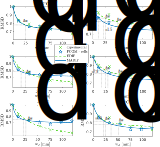
\includegraphics[width=0.95\textwidth]{Chapter_8/MADIF_temp_RMSD}
	\end{center}
	\caption{The \acf{madif} and the \acf{edif} based on the \acf{rmsd} 100 \unit{\kHz}.}
	\label{fig:madif_temp_rmsd}
\end{figure}
\begin{figure}
	\begin{center}
		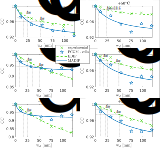
\includegraphics[width=0.95\textwidth]{Chapter_8/MADIF_temp_CC}
	\end{center}
	\caption{The \acf{madif} and the \acf{edif} based on the \acf{cc} 100 \unit{\kHz}.}
	\label{fig:madif_temp_cc}
\end{figure}
%% SECTION HEADER ///////////////////////////////////////////////////////////////////////////////////
\section{The numerical simulation of the \ac{gw} in the \ac{hsc} under various parameters}
\label{sec:parameters}

%% SECTION CONTENT ////////////////////////////////////////////////////////////////////////////////////
In addition to the previous analyses, a parametric study was conducted to determine the effects of various component parameters on \ac{gw} propagation in the \ac{hsc}. The following parameters were taken into account:
\begin{enumerate}
	\item The \ac{pzt} parameters:
	\begin{itemize}
		\item placement in relation to the core cell,
		\item charge constant,
		\item dielectric permittivity,
	\end{itemize}
	\item The \ac{cfrp} and the adhesive layer parameters:
		\begin{itemize}
		\item \ac{cfrp} fibre volume fraction,
		\item adhesive layer thickness,
		\end{itemize}
	\item The core parameters:
	\begin{itemize}
		\item core height and width,
		\item wall thickness,
		\item core rotation angle regarding to wave propagation.
	\end{itemize}
\end{enumerate}

\subsection{The \ac{pzt} parameters}
Computer simulations were conducted to determine the impact of \acp{pzt} placement relative to the core cell.
Seven transducer positions were considered, according to the schematic in Fig.~\ref{fig:pzt_place}(\textbf{b}).
The actuator and sensor position relative to the cell is identical to maintain the same wave propagation distance for each case.

From Fig.~\ref{fig:pzt_place}(\textbf{a}), it can be noticed that the highest amplitude of the \ac{s0} is obtained for the case with the \acp{pzt} placed in the middle of the cell.
The lowest amplitudes were obtained for the cases where the transducer midpoint lay on the core wall.
It is due to the higher stiffness underneath the \ac{pzt}, leading to less displacements.
In the case of the \ac{a0}, the amplitude of the signals for position \#2 and \#5 are much lower than the rest cases.
Since the transducers are permanently fixed to the structure and do not change their position during the monitoring period.
Nonetheless, the \acp{pzt} placement is worth considering to optimise the signals obtained.
\begin{figure}
	\begin{center}
		\includegraphics[width=0.95\textwidth]{Chapter_8/pzt_place}
	\end{center}
	\caption{The \acf{gw} propagation in the \acf{hsc} \textbf{(a)}, sensor responses for \textbf{(b)} different \acf{pzt} placement in relation to the core cell.}
	\label{fig:pzt_place}
\end{figure}

Changes in amplitude under the influence of different values of the piezoelectric charge constant and dielectric permittivity are presented in Fig.~\ref{fig:pzt_d} and ~\ref{fig:pzt_eps}, respectively.
Both parameters have a significant effect on the signal amplitude both the \ac{s0} and \ac{a0}.
The values do not just change with ambient temperature but also degrade over service time \cite{barzegar2001aging, deangelis2006p2o}.
Therefore, I suggest that a sensor self-diagnostic tool should be included in the \ac{shm} system. 
An \ac{emi}-based method could be a good solution as it was suggested for self-diagnostic of damaged transducers by Jiang et al. \cite{jiang2021electromechanical}.

\begin{figure}
	\begin{center}
		\includegraphics[width=0.95\textwidth]{Chapter_8/pzt_d}
	\end{center}
	\caption{The signal envelopes for different piezoelectric charge constants.}
	\label{fig:pzt_d}
\end{figure}

\begin{figure}
	\begin{center}
		\includegraphics[width=0.95\textwidth]{Chapter_8/pzt_eps}
	\end{center}
	\caption{The signal envelopes for different dielectric permittivities.}
	\label{fig:pzt_eps}
\end{figure}

\subsection{The \ac{cfrp} skin and the adhesive layer parameters}

The effect of the skin properties on wave propagation in the \ac{hsc} was analysed for different carbon fibre volume fractions in the composite.
This parameter affects the mode velocity due to the change in effective modulus of elasticity and density of the plate.
A small change in modulus of elasticity leads to significant signal differences within the interference of wave reflections as it can be observe in Fig.~\ref{fig:skin_volume}.
It affects the \ac{madif} determination since the full-length signal is taken into account.

\begin{figure}
	\begin{center}
		\includegraphics[width=0.95\textwidth]{Chapter_8/skin_volume}
	\end{center}
		\caption{Sensor responses in the \acf{hsc} for various fibre volume fractions in the range 45-50\%.}
	\label{fig:skin_volume}
\end{figure}

The effect of the adhesive layer thickness is presented in Fig.~\ref{fig:adhesive_thickness}.
The greater the adhesive thickness, the slower both modes propagate.
There is also a noticeable decrease in the \ac{a0} amplitude, while the \ac{s0} amplitude barely changes.
It is because the \ac{a0} displacements are mainly out-of-plane, so more energy of the wave leaks into the adhesive, and it is attenuated in low-stiffness material.

\begin{figure}
	\begin{center}
		\includegraphics[width=0.95\textwidth]{Chapter_8/adhesive_thickness}
	\end{center}
	\caption{Sensor responses in the \acf{hsc} for various adhesive thicknesses in the range 200-500 \(\mu\)m.}
	\label{fig:adhesive_thickness}
\end{figure}

\subsection{The core parameters}
In the study of the core geometry influence on wave propagation in \ac{hsc}, four parameters were considered:
\begin{itemize}
	\item core height \(g=[10.5,\,12.5,\,14.5,\,16.5,\,18.5]\) \unit{\mm};
	\item core width \(l_1=[5.0,\,6.0,\,7.0,\,8.0,\,9.0]\) \unit{\mm};
	\item wall thickness \(w_c=[100,\,150,\,200,\,250,\,300]\) \unit{\micro\m};
	\item core rotation angle regarding to wave propagation [\ang{0}, \ang{15}, \ang{30}, \ang{45}, \ang{60}, \ang{75}, \ang{90}].
\end{itemize}

From the signal envelopes shown in Fig.~\ref{fig:core_height}, \ref{fig:core_size}, \ref{fig:core_thickness} and \ref{fig:core_rotation} it can be seen that the analysed parameters mainly affect the \ac{a0}. 
In contrast, for the \ac{s0}, only the amplitude changes, except for the reduction in velocity by the increase in wall thickness.

It should be mentioned that all parameters are invariable during the use of the structure and are independent of changing environmental conditions.
Therefore, the core heights and wall thicknesses are set with the dimensions tolerance received from the supplier.
The cell can easily be deformed before bonding to the skin due to the low in-plane stiffness of the core.
Thus for better accuracy, the cell width can be assumed as an average measurement value taken after joining the core with the skin.
The angle of rotation can also be corrected after the components bonding.
\begin{figure}
	\begin{center}
		\includegraphics[width=0.95\textwidth]{Chapter_8/core_height}
	\end{center}
	\caption{Sensor responses in the \acf{hsc} for the various core heights in the range 10.5-18.5 \unit{\mm}.}
	\label{fig:core_height}
\end{figure}

\begin{figure}
	\begin{center}
		\includegraphics[width=0.95\textwidth]{Chapter_8/core_size}
	\end{center}
	\caption{Sensor responses in the \acf{hsc} for the various cell widths in the range 5.0-9.0 \unit{\mm}.}
	\label{fig:core_size}
\end{figure}

\begin{figure}
	\begin{center}
		\includegraphics[width=0.95\textwidth]{Chapter_8/core_thickness}
	\end{center}
	\caption{Sensor responses in the \acf{hsc} for the various wall thicknesses in the range 100-300 \unit{\micro\m}.}
	\label{fig:core_thickness}
\end{figure}

\begin{figure}
	\begin{center}
		\includegraphics[width=0.95\textwidth]{Chapter_8/core_rotation}
	\end{center}
	\caption{Sensor responses in the \acf{hsc} for the various core orientations.}
	\label{fig:core_rotation}
\end{figure}

\subsection{The \ac{madif} for the double-skin \ac{hsc}}

Finally, computer simulations were conducted to determine the \ac{madif} for a structure with a core between two skins.
The single-skin \ac{fcgm} from the previous analyses was supplemented with a \ac{cfrp} plate and also bonded to the core by the adhesive layer.
Two transducers were attached to the top skin as before.
Due to the impossibility of enlarging the damage in a closed-form structure, no experimental measurements were carried out.
Two damage cases were considered in the simulations: (i) interface elements removed from the upper side (the skin with the sensor attached), and (ii) interface elements removed from the bottom side.

Fig.~\ref{fig:madif_2skins}\textbf{(a)} presents the \ac{rmsd}-based \ac{madif} for a double-skin panel with the functions obtained for a single-skin for comparison.
Substantial differences between the double- and single-skin panels can be observed.
In addition, the placement of the damage has also influence on the index slope.
Similar changes in the \ac{madif} can be observed for \ac{cc}, as shown in Fig. ~\ref{fig:MADIF_2skins}\textbf{(b)}.
Although to a lesser extent than the previous index. 
The \ac{rmsd} values ratio single- to double-skin panel for the most significant damage is about 1.5, while the relevant ratio based on \ac{cc} is about 1.08.
\begin{figure}
	\begin{center}
		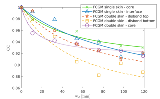
\includegraphics[width=0.95\textwidth]{Chapter_8/MADIF_2skins}
	\end{center}
	\caption{Comparison of the \acf{madif} for single-skin and double-skin panels based on \textbf{(a)}the \acf{rmsd} and \textbf{(b)} the \acf{cc}.}
	\label{fig:madif_2skins}
\end{figure}
\section{Conclusions}
\label{sec:conclusionsTemp}
This chapter presented a parametric study to obtain temperature-dependent \ac{madif} and determine the influence of various parameters of structural components on \ac{gw} propagation in \ac{hsc}.

The \ac{madif} obtained numerically for different ambient temperatures agree very well with the experimental results, especially for temperatures around the reference one.
The absolute error increases with the higher difference in temperature.
It is probably because the assumed linear model is not sufficient enough.

During the analysis, it was shown that the \ac{hsc} is a very complex structure and that all the parameters of each component affect the amplitude or velocity of the wave propagated in this structure.
In the future, it would be essential to develop an effective tool to determine the material properties and geometry of the structure in order to correspond the model to the monitored sample more accurately.
Such a tool based on an optimisation algorithm has been developed for a woven fabric reinforced composites by Kudela et al. \cite{kudela2020elastic}.

Computer simulations were also conducted to determine the \ac{madif} for a double-skin structure.
The function, similar to that of a single-skin panel, satisfies the conditions for damage estimation.
It is a monotonic function for the entire damage range, and its values are even more extensive than in the first case.